%%%%%%%%%%%%%%%%%%%%%%%%%%%%%%%%%%%%%%%%%%%%%%%%%%%%%%%%%%%%%%%%%%%%%
% LaTeX Template: Project Titlepage Modified (v 0.1) by rcx
%
% Original Source: http://www.howtotex.com
% Date: February 2014
% 
% This is a title page template which be used for articles & reports.
% 
% This is the modified version of the original Latex template from
% aforementioned website.
% 
%%%%%%%%%%%%%%%%%%%%%%%%%%%%%%%%%%%%%%%%%%%%%%%%%%%%%%%%%%%%%%%%%%%%%%

\documentclass[12pt]{article}
\usepackage[a4paper]{geometry}
\usepackage[myheadings]{fullpage}
\usepackage{fancyhdr}
\usepackage{lastpage}
\usepackage{graphicx, wrapfig, subcaption, setspace, booktabs}
\usepackage[T1]{fontenc}
\usepackage[font=small, labelfont=bf]{caption}
\usepackage{fourier}
\usepackage[protrusion=true, expansion=true]{microtype}
\usepackage[english]{babel}
\usepackage{sectsty}
\usepackage{url, lipsum}
\usepackage{tgbonum}
\usepackage{hyperref}
\usepackage{xcolor}

\newcommand{\HRule}[1]{\rule{\linewidth}{#1}}
\onehalfspacing
\setcounter{tocdepth}{5}
\setcounter{secnumdepth}{5}



%-------------------------------------------------------------------------------
% HEADER & FOOTER
%-------------------------------------------------------------------------------
%\pagestyle{fancy}
%\fancyhf{}
%\setlength\headheight{15pt}
%\fancyhead[L]{Student ID: 1034511}
%\fancyhead[R]{Anglia Ruskin University}
%\fancyfoot[R]{Page \thepage\ of \pageref{LastPage}}
%-------------------------------------------------------------------------------
% TITLE PAGE
%----------------------------------------------------------------- --------------

\begin{document}

\fontfamily{cmr}\selectfont

\title{ \normalsize \textsc{}
		\\ [2.0cm]
		\HRule{0.5pt} \\
		\LARGE \textbf{De-novo Transcriptome assembly, annotation and evaluation pipeline report
		\HRule{2pt} \\ [0.5cm]
		\normalsize \today \vspace*{5\baselineskip}}
		}

\date{}

\author{
		IPMB, Universit\"at Heidelberg \\
		}

\maketitle

\newpage

\tableofcontents

\section{De novo tanscriptome assembly, annotation and evaluation pipeline}

\begin{figure}[h]
    \centering
    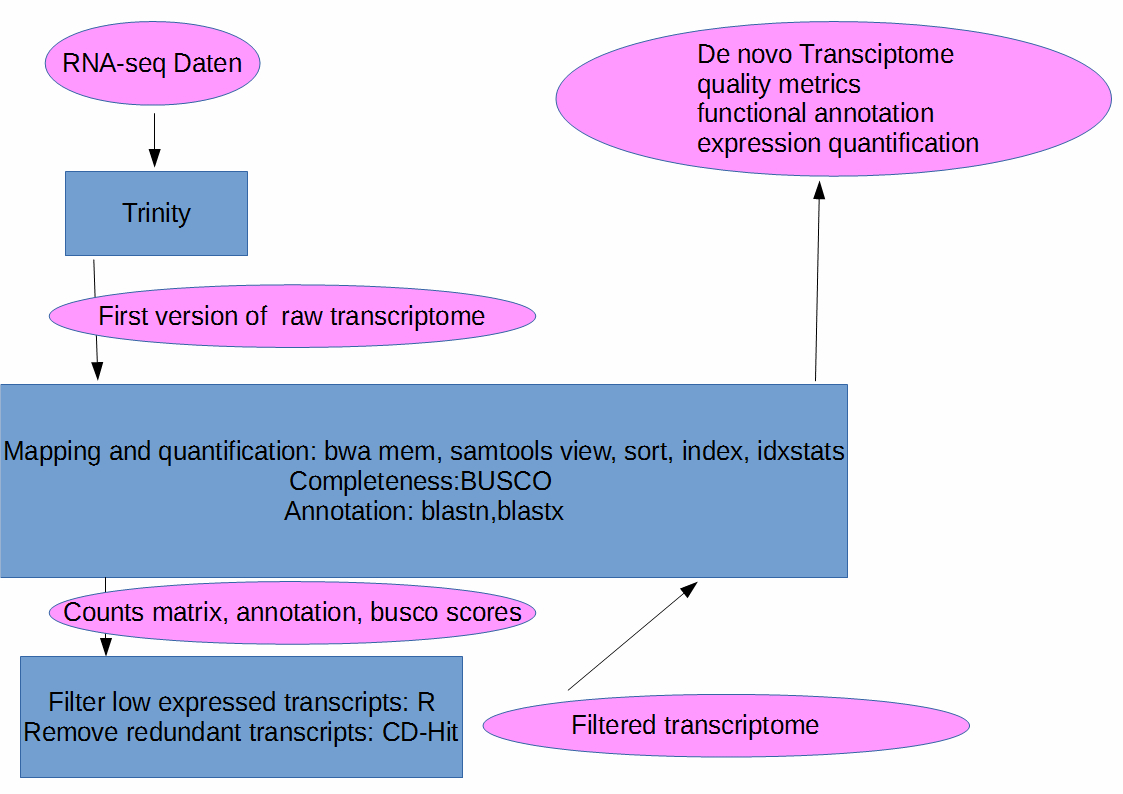
\includegraphics[width=12cm]{pipeline}
    \caption{Pipeline components}
    \label{fig:pipeline}
\end{figure}



\subsection{De novo assembly and postprocessing}

The tissue reads were pulled together to assemble a de-novo transcriptome for the O.oenante. This was made with Trinity \cite{trinity}, version 2.6.5, with the options $--normalize\_reads$, $--normalize\_max\_read\_cov$ 50 and $--single$. \\

We removed redundant transcripts with CD-Hit-EST \cite{cdhit,cdhit1} (sequence similarity of 0.9). We programmed an R script to filter out assembling artefacts. We defined as artefacts, transcripts that were low expressed throughout all samples of a species. All discarded transcripts accounted for at most !!thresh!! percentage of the reads originally mapped to the raw transcriptome. This way we obtained a compact, non-redundant transcriptome for the studied species.\\ 

\subsection{Completeness}  

Benchmarking Universal Single Copy Orthologs (BUSCO)\ cite{busco} version 3.0.2 was used to estimate how complete the new transcriptome is, based on the database !!buscodb!!. 

\subsection{Mapping and expression quantification}

Tissue reads were remapped to the new transcriptome using the mem algorithm of bwa, version 0.7.12 \cite{bwamem}. Bwa mem allows and flags supplementary alignments. \\

Expression was quantified per transcript and per gene with featureCounts \cite{featureCounts} (Release 1.6.4), ignoring multi-mapping and multi-overlapping reads. As normalized transcript expression, we calculated RPKMs. For normalized gene expression, we used DESeq2 normalized read counts (since the actual gene length for genes with several isoforms remains unknown to us).

\subsection{Annotation}

Transcripts were annotated to the !!anndb!! database, using !!blast!!. Best hit (maximum Bitscore) was selected as the annotation for the transcript from all hits with Percentage Identity greater equals to !!blastpid!!. \\

Based on the annotation, we summarized all transcripts with a unique Gene\_Symbol into a single gene. Unnanotated transcripts were summarized into genes, following Trinity notation for genes/isoforms.

\section{Results}

The analyzed data is summarized on table \ref{table:labs}

!!labs!! 

\subsection{Postprocessed denovo transcriptome}

Some common assembly statistics (e.g. N50) are shown in Table \ref{table:trsstats}. Figure \ref{fig:lengthdist} shows the de novo transcripts log-length distribution compared to some already published transcriptome.\\ 

!!table:trsstats!!

\begin{figure}
    \centering
    \includegraphics[width=12cm]{lengthdist.pdf}
    \caption{Transcripts length distribution}
    \label{fig:lengthdist}
\end{figure}


\subsection{Quality metrics}
The number and percentage within brackets of original reads that were remapped/unmapped to the assembled transcriptome are shown in Figure \ref{fig:mapstats} and Table \ref{table:mapstats} 

!!table:mapstats!!

\begin{figure}
    \centering
    \includegraphics[width=12cm]{mapping}
    \caption{Mapping statistics of raw reads to postprocessed transcriptomes}
    \label{fig:mapstats}
\end{figure}

The BUSCO score for each species is shown in Table \ref{table:buscostats} and Figure \ref{fig:buscostats}

\begin{figure}
    \centering
    \includegraphics[width=12cm]{buscostats}
    \caption{BUSCO score for postprocessed transcriptomes}
    \label{fig:buscostats}
\end{figure}

!!table:buscostats!!

The number of annotated transcripts to the !!anndb!! database is show in Table \ref{table:annstats} and Figure \ref{fig:annstats}. 

!!table:annstats!!
\begin{figure}
    \centering
    \includegraphics[width=12cm]{annstats_pid!!blastpid!!}
    \caption{Annotation statistics of de novo transcripts to !!anndb!! database}
    \label{fig:annstats}
\end{figure}

!!fig:swporgs!!

\newpage
\bibliographystyle{plain}
\bibliography{ref}

\end{document}